\begin{figure}[t]
    \centering
    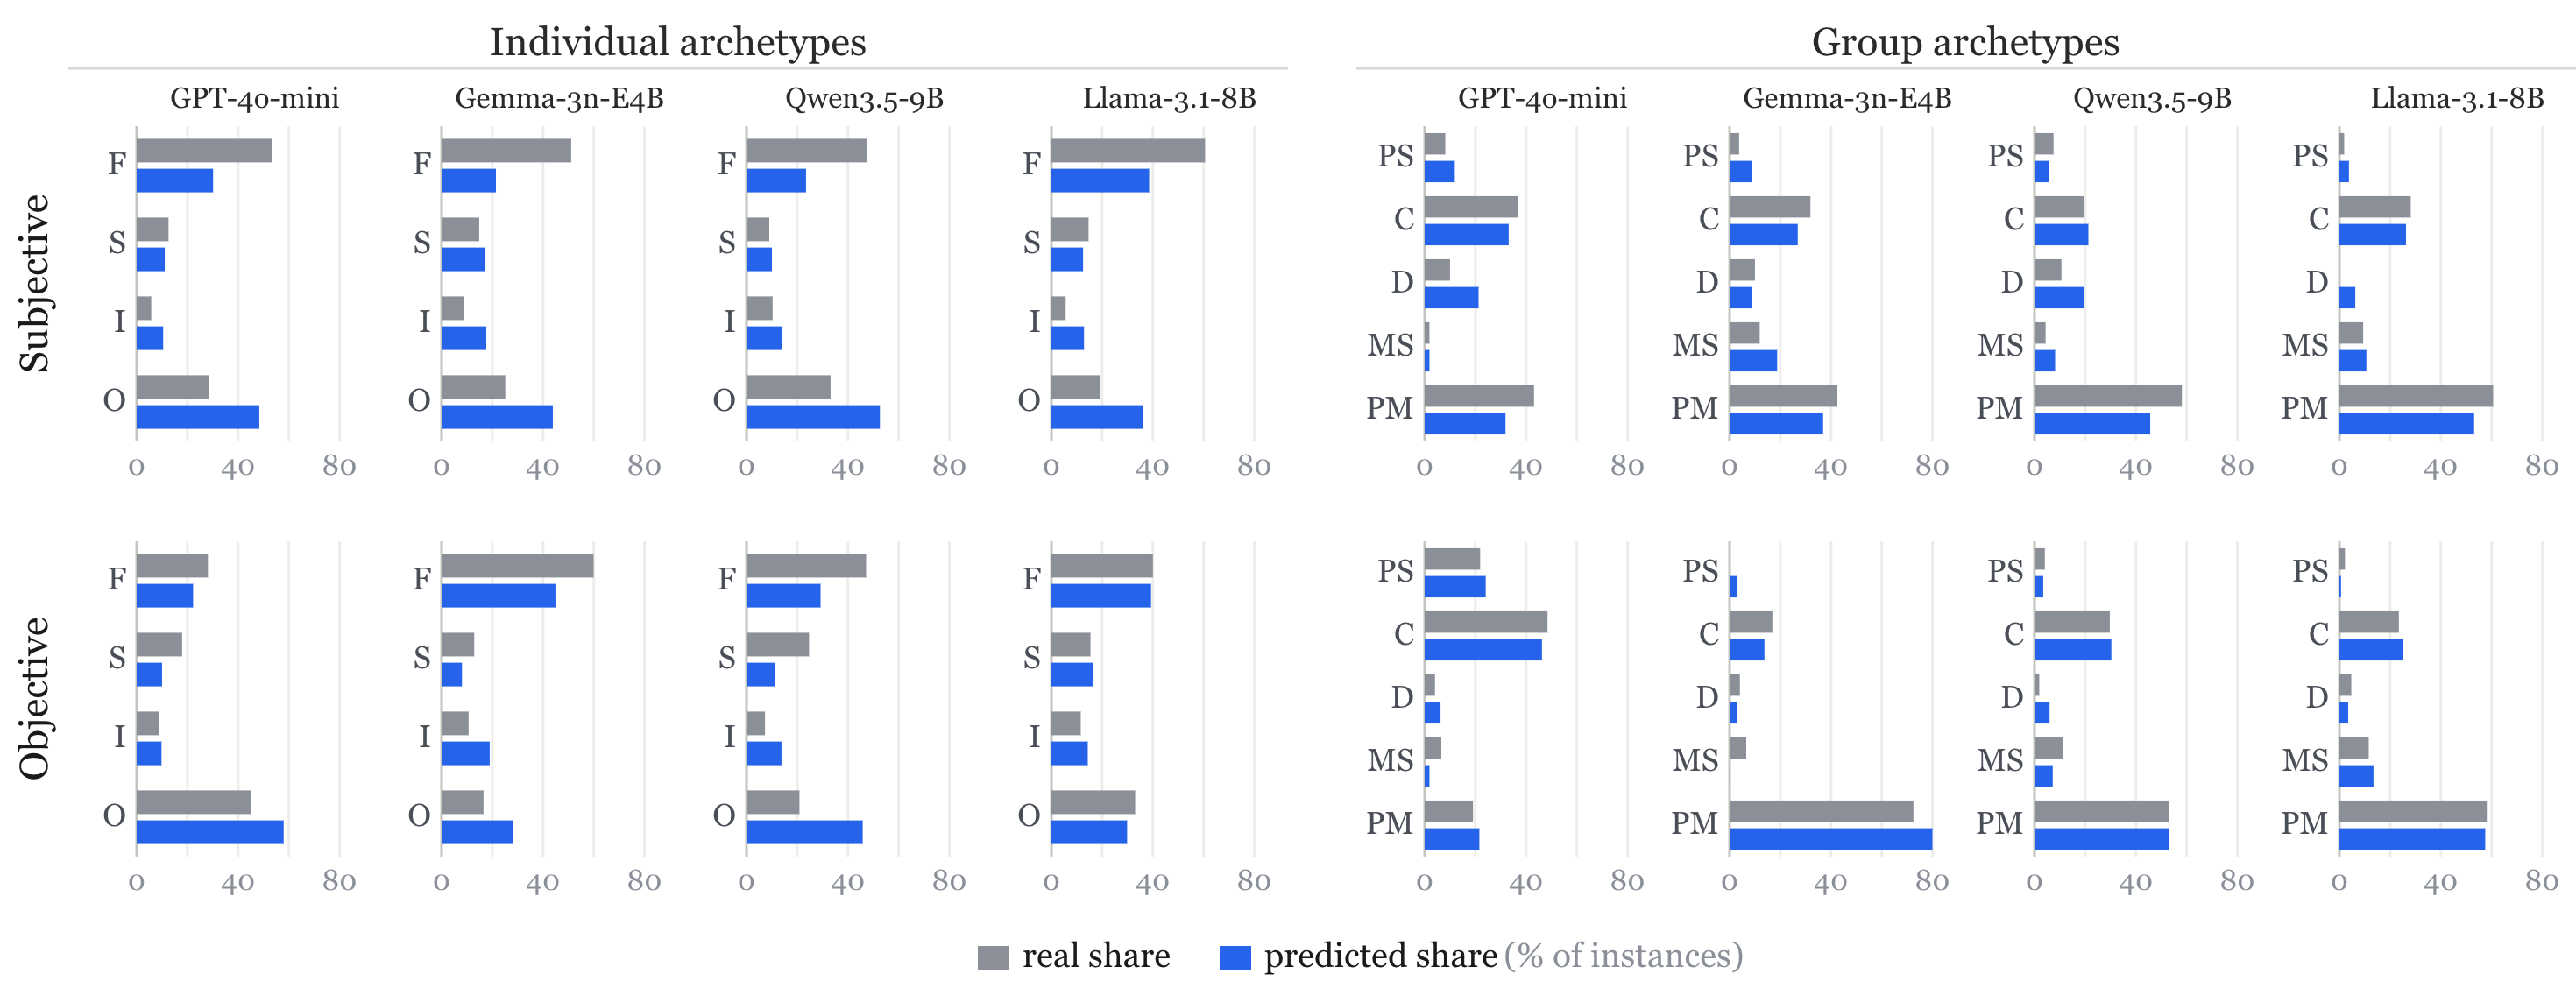
\includegraphics[width=0.99\textwidth]{main/Figures/main_06_archetype_distribution.png}
\caption{\textit{Distribution of Individual and Group Archetypes.} Shares
of individual and group archetypes are shown as horizontal bars (F~(Frozen), S~(Switcher), I~(Intermittent), O~(Oscillating); PS~(Persistent Split), C~(Convergence), D~(Divergence), MS~(Majority Switch), PM~(Persistent Majority)). The shares are computed on the held-out test set questions using the in-distribution random graphs by running stochastic rollout of the fitted Discrete Three couplings model from the real $s(0)$ for $8$ rounds, in which each agent's next opinion is sampled as $s_i(t{+}1)=+1$ with probability $\sigma(h_i(t))$ rather than thresholded at at probability $1/2$. \label{fig:macrostate_distribution}}
\end{figure}


\subsection{Distributions of Archetypes}\label{sec:results_distributions}

\textit{Predicting the Distribution of Group Archetypes.} We also investigate whether the fitted model, run from the real initial opinions $s(0)$ as a roll-out, produces communities that look like the real ones in aggregate. Because the fitted rule is a probability rather than a decision, we sample each agent's next opinion from $P(s_i(t{+}1)=+1)=\sigma(h_i(t))$, where $h_i(t)$ is the fitted logistic argument of Section~\ref{sec:method}, instead of thresholding it at $\sigma = 1/2$, so that the rollouts carry the noise the rule assigns. Figure~\ref{fig:macrostate_distribution} compares the shares of the individual and group archetypes of Section~\ref{sec:macrostates_microstates} between the held-out communities and these rollouts (for details on the roll-outs, see Appendix~\ref{apdx:rollouts}).

\textit{Individual and Group Archetypes.} In Figure~\ref{fig:macrostate_distribution}, the group archetype shares deviate by only $\sim\!3$ points for objective questions and $\sim\!5$ points for subjective questions (mean absolute deviation). The largest single gap is $\sim\!10$ points (Qwen3.5-9B subjective, Persistent Majority) and the two dominant classes correct in every cell. Meanwhile, the model inflates the oscillator count in individual archetypes, but this appears to largely cancel out in the group archetype distributions. The fitted dynamics therefore reproduce the collective statistics even when they misstate how often an individual agent changes its mind.  We note that this observation demonstrates that the fitted dynamics produce the right mix of outcomes, not that they place a given group in the right archetype.

\textit{Reproducibility of Group Trajectories.} We observe that group trajectories are only partly predictable. We run each group as four episodes with identical personas, graph and question that differ only in sampling randomness. We compare how often one episode's group archetype matches the other samples taken with the identical personas, graph, and question. Figure ~\ref{fig:predictability_macro_subjective_test_J03_cv_row} in Appendix~\ref{apdx:replica_predictability} reports this ceiling. Episodes frequently disagree on the group archetype, which is why we evaluate the fitted rule at the level of the distribution.

